% !TEX root = /home/jd18380/Documents/compass_yr1/Stat_methods/Portfolio/Section_2/main.tex
\documentclass[a4paper]{article}

%% Language and font encodings
\usepackage[english]{babel}
\usepackage[utf8x]{inputenc}

\usepackage{booktabs}
\usepackage{tabu}
\usepackage[T1]{fontenc}
\usepackage{subfig}

%% Sets page size and margins
\usepackage[a4paper,top=2cm,bottom=3cm,left=3cm,right=3cm,marginparwidth=2.75cm]{geometry}
%% Useful packages
\usepackage{amsmath}
\usepackage{amsfonts}
\usepackage{amssymb}
\usepackage{bm}
\usepackage{xcolor}
\DeclareMathOperator*{\argmax}{arg\!\max}
\DeclareMathOperator*{\argmin}{arg\!\min}
\usepackage[toc,page]{appendix}
\usepackage{graphicx}
%\usepackage{apacite}
\usepackage[colorinlistoftodos]{todonotes}
\usepackage[colorlinks=true, allcolors=blue]{hyperref}
\usepackage{cleveref}

\newtheorem{theorem}{Theorem}[section]
\newtheorem{corollary}{Corollary}[theorem]
\newtheorem{lemma}[theorem]{Lemma}
\newtheorem{definition}{Definition}[section]
\newtheorem{question}{Question}[subsection]

\newcommand{\yi}{y_{i}}
\newcommand{\gxi}{g_{\bm{x}_{i}}}
\newcommand{\gx}{g_{\bm{x}}}
\newcommand{\ei}{\epsilon_{i}}
\newcommand{\E}{\mathbb{E}}
\newcommand{\wls}{\bm{w}_{LS}}
\newcommand{\wlsr}{\bm{w}_{LS-R}}
\newcommand{\wmap}{\bm{w}_{MAP}}
\newcommand{\xui}{\bm{x}_{i}}
\newcommand{\prls}{f(\xui ; \wls)}
\newcommand{\prlsv}{f(\bm{x} ; \wls)}
\newcommand{\V}{\text{Var}}
\newcommand{\y}{\bm{y}}
\newcommand{\x}{\bm{x}}
\newcommand{\w}{\bm{w}}
\newcommand{\F}{\bm{\phi}}
\newcommand{\I}{\bm{I}}
\newcommand{\X}{\bm{X}}
\newcommand{\K}{\bm{K}}
\newcommand{\yh}{\hat{y}}
\newcommand{\dpost}{\Delta \textit{posterior}}
\newcommand{\dprior}{\Delta \textit{prior}}
\renewcommand{\t}{\bm{t}}
\newcommand{\W}{\bm{W}}
\newcommand{\Wls}{\bm{W}_{LS}}
\newcommand{\muhatk}{\hat{\mu}_{k}}


\title{Statistical Methods: Portfolio 3}
\author{By Henry Bourne}
\date{}

\begin{document}
\maketitle


% \begin{abstract}
%     In this document we will summarize content from the first 4 lectures from the Statistical methods course (at Compass, University of Bristol). These lectures cover content on using statistical methods for decision-making.
% \end{abstract}

\section*{Question 0}
E

\section*{Question 1}

\subsection*{1.1}
The answer is c or d as this line goes roughly through the class means and when the data points are projected onto the embedding vector (for either of the directions) it appears as though the between-class scatterness will be maximized and the within-class scatterness minimized as points from the negative/positive class will be close together and the class means in the embedding will be fairly centrally located (within their classes). For comparison we can argue that the opposite would be true for directions a and b, where points from both classes will not be separated (class-wise) in the embedding and the furthest points from a given class to its class mean will be larger than we had with embedding vectors in directions c or d. 

\subsection*{1.2}
We can construct a likelihood function over the entire dataset:
\begin{equation}
    L(\bm{\mu},\bm{\Sigma}) := \prod_{i=1}^{n} p(\xui | \bm{\mu}, \bm{\Sigma}) = \prod_{i=1}^{n} N_{\xui}(\bm{\mu},\bm{\Sigma})
\end{equation}
ie. all the points are iid. normally distributed (have same mean and covariance matrix) where $\bm{\Sigma}_{ML}$ maximizes the above likelihood.

Let's take the decomposition to be the eigen-decomposition of $\bm{\Sigma}_{ML}$, then $\bm{\mu}_{1}$ is an eigenvector of $\bm{\Sigma}_{ML}$ with corresponding eigenvalue $D_{1}$. Note that $D_{1} > D_{2}$ which means the eigenvector $\bm{u}_{1}$ corresponds to the direction of the largest variance in the data, hence must correspond to direction a or b. 

\section*{Question 3}
Recall the soft margin SVM:
\begin{align}
    \text{Minimize} \: \: || \w '||^{2} + \sum_{i \in D} \epsilon_{i} \\
    \text{Subject to} \: \: \forall i, y_{i} \cdot f(\xui ; \w) + \epsilon_{i} \geq 1, \epsilon_{i} \geq 0
\end{align}
We can modify the objective function such that it penalizes False Negatives (FN) by making FNs 1000 times more costly by rewriting the objective function as:
\begin{equation}
    \text{Minimize} \: \: || \w ' ||^{2} + \sum_{i \in D} (1000 \cdot I(y_{i}=1) + (1-I(y_{i}=1))  )\cdot \epsilon_{i}
\end{equation}
where $I(y_{i}=1)$ is the indicator function that is one when $y_{i}=1$ (ie. when wrongly classifying would lead to a FN) it multiplies the cost times 1000. So, during optimization we will have attributed a 1000x cost to giving a FN, meanwhile the cost of a FP stays as is (a 1000th of the cost).

\section*{Question 4}
\subsection*{4.1}
B
\subsection*{4.2}
The factorization of $p(y,x^{(1)},x^{(2)},x^{(3)},x^{(4)})$ according the to graph is:
\begin{equation}
    p(y) \cdot p(x^{(1)}|y) \cdot p(x^{(2)}|y,x^{(1)}) \cdot p(x^{(3)}|x^{(2)}) \cdot p(x^{(4)}|x^{(1)}) 
\end{equation}
The conditional independencies encoded by this graph are:
\begin{align}
    x^{(2)} \bot x^{(4)} | y,x^{(1)} \\
    x^{(3)} \bot y,x^{(1)},x^{(4)} | x^{(2)} \\
    x^{(4)} \bot y, x^{(2)}, x^{(3)} | x^{(1)}
\end{align}
And no we should just use $x^{(1)}$ and $x^{(2)}$ as given these two features we have from our conditional independencies that $x^{(3)}$ and $x^{(4)}$ are independent of y, we also have that our prediction function:
\begin{align}
    p(y|x^{(1)},x^{(2)},x^{(3)},x^{(4)}) &{} = \frac{p(y) \cdot p(x^{(1)}|y) \cdot p(x^{(2)}|y,x^{(1)}) \cdot p(x^{(3)}|x^{(2)}) \cdot p(x^{(4)}|x^{(1)})}{p(x^{(1)},x^{(2)},x^{(3)},x^{(4)})} \\
    &\propto p(y) \cdot p(x^{(1)}|y) \cdot p(x^{(2)}|y,x^{(1)})
\end{align}
Therefore to formulate a prediction for y we only need $x^{(1)}$ and $x^{(2)}$.
\newpage
\begin{appendices}


% \section{Proofs}

% \subsection{---} \label{Proofs:}



%\newpage
\section{Homeworks}
\subsection{For Section 1}

\begin{question}\label{question:graph-equivelance}
    \textbf{Show equivalence between the factorization and conditional independence over G in the Scores of units example:} \\
    First we will create G using the following factorization:
    \begin{equation}
        p(\text{Maths}, \text{SM}1, \text{Python}, \text{ML}) \propto g_{1}(\text{Maths}, \text{SM}1) \cdot g_{2}(\text{Python}, \text{ML}, \text{SM}1)
    \end{equation}
    The graph corresponding to this factorization is:
    \begin{figure}[h]
    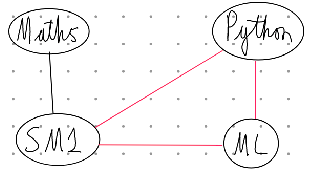
\includegraphics[width=\textwidth/2]{images/factor_graph.png}
    \centering
    \end{figure}
    Where in black is the edges corresponding to the clique given by the first factor and in red the edges corresponding to the clique given by the second factor. The conditional independencies encoded by this graph are:
    \begin{enumerate}
        \item Maths $\bot$ Python $|$ SM1
        \item Maths $\bot$ Python $|$ SM1, ML 
        \item Maths $\bot$ ML $|$ SM1
        \item Maths $\bot$ ML $|$ SM1 , Python
        \item Maths $\bot$ ML, Python $|$ SM1
    \end{enumerate}
    Which are all the conditional independencies of $p(\text{Maths}, \text{SM}1, \text{Python}, \text{ML})$. 

    Now we will create G using all the conditional independencies, which are:
    \begin{enumerate}
        \item Maths $\bot$ Python $|$ SM1
        \item Maths $\bot$ Python $|$ SM1, ML 
        \item Maths $\bot$ ML $|$ SM1
        \item Maths $\bot$ ML $|$ SM1 , Python
        \item Maths $\bot$ ML, Python $|$ SM1
    \end{enumerate}
    The graph we get is the same as before, and reading the graph its clear that it encodes the factorization of $p(\text{Maths}, \text{SM}1, \text{Python}, \text{ML})$. Hence, shown.
\end{question}

\subsection{For Section 2}
\begin{question}
    \textbf{Suppose graph G encodes all conditional independencies in your Gaussian distribution $p(\x)$. Let's say G contains 3 edges and 5 nodes. How many non-zero elements are there in inverse covariance matrix of p?:} \\
    There are 25 entries in $\bm{\Theta}$ and in the adjacency matrix of G (also with 25 entries) there are 6 non-zero (ie. equal to 1) entries hence only 6 entries in $\bm{\Theta}$ that are non-zero (from \cref{equation:adjacency-Theta}). 
\end{question}

\begin{question}\label{question:logistic-regression}
    \textbf{In \cref{subsubsection:Logistic-Regression} we constructed a logistic regression from our simple Markov network model where $\hat{\bm{\beta}}, \hat{\beta_{0}} = \argmax_{\bm{\beta}, \beta_{0}} \sum_{i=1}^{n} \log(p(y_{i}|\xui;\bm{\beta},\beta_{0}))$ show that this is the same logistic regression we talked about in portfolio 3:} \\
    Note that we can write:
    \begin{equation}
        p(y=-1| \x) = 1 / (1+ \frac{p(\x|y=+1)p(y=+1)}{p(\x|y=-1) p(y=-1)})
    \end{equation}
    And for $p(y=-1|\x)$ the same is true but with the inverse of the ratio of the densities. We can rewrite this more generally as:
    \begin{equation}
        p(y | \x; \bm{\beta}, \beta_{0}) = \sigma(f(\x;\bm{\beta}, \beta_{0}) \cdot y)
    \end{equation}
    where $f(\x;\bm{\beta}, \beta_{0}) = log( [p(\x|y=+1)p(y=+1)] / [p(\x|y=-1) p(y=-1)] )$. Hence we can rewrite our MLE as the logistic regression:
    \begin{equation}
        \hat{\bm{\beta}}, \hat{\beta_{0}} = \argmax_{\bm{\beta}, \beta_{0}} \sum_{i=1}^{n} \log (\sigma(f(\xui;\bm{\beta}, \beta_{0}) \cdot y_{i}))
    \end{equation}
    Which is the same logistic regression we had in portfolio 3.
\end{question}


\subsection{For Section 3}
\begin{question}
    \textbf{Given the simple Bayesian Network model described in \cref{section:Bayesian-Network}, however, now with one additional node $X'$ which has one inbound directed edge from $X^{(1)}$. Given this Bayesian Network for a classification task, should you include feature $X'$ for classification? and why?} \\
    To be able to solve the classification problem we would like to find $p(Y|X)$ which for this Bayesian Network is equal to:
    \begin{equation}
        P(Y|X) = \frac{\prod_{i} P(X^{(i)} | Y) P(Y)P(X' | X^{(1)}) }{P(X)}
    \end{equation}
    Hence, we should include feature $X'$ for classification as our factorization and therefore prediction depends on it. 
\end{question}


\end{appendices}

% \small
% \bibliographystyle{plain}
% \bibliography{refs}

\end{document}